\documentclass[times, utf8,projekt]{fer}
%\usepackage{titlesec}
\graphicspath{ {./figures/} }
\setcitestyle{numbers}
\usepackage{color}
\usepackage{hyperref} 
\usepackage[nodayofweek,level]{datetime}
%\usepackage[numbers,square]{natbib}
\usepackage{etoolbox}
\makeatletter
\patchcmd{\chapter}{\if@openright\cleardoublepage\else\clearpage\fi}{}{}{}
\makeatother

%\titleformat{\chapter}[display]
%  {\normalfont\bfseries}{}{0pt}{\Large}

\begin{document}
\title{Stvaranje grafa, Clustering}
\maketitle
%općenit opis podjele rada kako bismo objasnili motivaciju naziva poglavlja koja imamo
Nakon početnog grupnog istraživanja grafova znanja i termina BKT, DKT, IRT i sl., dio grupe se odvojio na dubinsko istraživanje BKT-a, a dio na proučavanje koncepata stvaranja grafa znanja. U kasnijoj fazi, nakon pronalaska i refaktoriranja obećavajućeg modela preporuka zadataka pod nazivom ExRec, definiran je i zadatak vizualnog grupiranja zadataka koji pripadaju različitim konceptima. Među zadacima stvaranja grafa i grupiranja primijećene su velike korelacije; njihovo nadovezivanje i upotpunjavanje.

\chapter{Stvaranje grafa}
\section{Početna istraživanja}
Većina prvih proučenih radova i modela je napuštena zbog nepoklapanja s glavnom idejom našeg projekta, prevelike matematičke kompliciranosti ili kompleknosti računarske izvedbe te zbog namjernog ili nenamjernog uskraćivanja informacija o pozadini funkcionalnosti u objavljenim radovima.\newline
\newline
\subsection{Obrada prirodnog jezika}
Početna istraživanja mogućnosti stvaranja grafa odvela su nas u smjeru metoda s korištenjem NLP-a (engl. \textit{natural language processing}). Iako je smjer ocijenjen kao prezahtjevan za potrebe projekta, proučene su osnovne funkcionalnosti Python biblioteka koje olakšavaju takve postupke - spaCy, networkX, seaborn \citep{ct1}. NetworkX je kasnije korišten za vizualizaciju grafova u BKT-u, kao u i Lentil pokušajima grupiranja zadataka po konceptima.\newline
\newline
\subsection{K12EduKG}
Za edukacijske aplikacije pronađen je K12EduKG, sustav automatske konstrukcije grafa znanja gdje čvorovi i veze predstavljaju međusobno povezane koncepte \citep{ct2}, no nejasan je način pretakanja te ideje u kod koji bi odgovarao našem problemu. Autori daju premalo iskoristive informacije. Odlučeno je nastaviti istraživanje u drugačijim smjerovima.\newline
\newline
Novi smjerovi istraživanja od tog trenutka uključuju Deep Generative Models i GraphRNN. Proučeni su općeniti koncepti metoda nepovezani s edukacijskim aplikacijama kako bi poslužili kao inspiracija za nadogradnju na naš problem.\newline
\newline
\subsection{Deep Generative Models}
Model je temeljen na klasi modela grafičkih neuronskih mreža (engl. \textit{graph nets}). Uči reprezentaciju grafova; čvorova i veza prema propagaciji informacije. Sekvencijalno generira nove strukture (čvor ili vezu). Generiranje je slijed odluka o dodavanju gradivnih dijelova strukture predstavljen vjerojatnostima u zasebnim modulima:
\begin{itemize}
	\item{dodati čvor ili ne,}
	\item{dodati vezu ili ne,}
	\item{zabrati jedan čvor da se spoji s nekim novim.}
\end{itemize}
Drugačiji poredak struktura označava različite odluke.
Za graf se koristi tzv. vektor ugradnje čvorova (engl. \textit{node embedding vector}). Računaju se “skrivena stanja” iz ulaza čvorova i propagiraju se grafom za dobivanje informacije lokalnog susjedstva. Vektor poruke računa se za svaku vezu (pomoću potpuno povezane neuronske mreže, GRU ili LSTM) pa svaki čvor dobiva tu informaciju i osvježava svoj prikaz \citep{ct3}.
Spominje se i mogućnost uključivanja uvjetne informacije za proces generiranja. Kao i u prethodnom primjeru, autori ne objavljuju sve potrebne informacije. Oblik vektora ostaje nepoznat, kao i način izračuna "skrivenih stanja" za vektor ugradnje.\newline
\newline
\subsection{Graph RNN}
Autoregresivni model. Autoregresivni modeli su sekvencijalni modeli, ali i s unaprijednom propagacijom; generativni, ali i pod nadzorom. Imaju velik potencijal kao alternativa povratnim neuronskim mrežama i GAN-ovima, generativnim suparničkim mrežama (engl. \textit{generative adversarial newtorks}) za obavljanje generiranja \cite{ct4}. Izlaz su im prediktivne uvjetne vjerojatnosti $P(x_{t+1} | x_1, …, x_t)$. Uvjetovanje je moguće samo na podatcima (ne npr. na šumu kao kod GAN-ova).
Konkretno, kod Graph RNN dijelovi matrice susjedstva generiraju se sekvencijalno (npr. jedan po jedan stupac) pomoću RNN.
Daljnijm proučavanjem prepoznati su mnogi nedostaci ovog modela. Složenost je O($N^2$), gdje je $N$ broj čvorova. Nadalje, zbog sekvencionalnosti, dva bliska čvora grafa mogu biti jako udaljeni u procesu generiranja u RNN što otežava performanse. Prilično je bitno osigurati invarijantnost na permutacije u čvorovima zbog izračuna vjerodostojnosti. Jedan od nedostataka pristupa svakako je i korištenje BFS algoritma (engl. \textit{breadth-first search}) za redanje čvorova u grafu; vrlo efikasnog računski, ali neoptimalnog.\newline
\newline
\section{Graph Recurrent Attention Networks}
\subsection{Općenito o GRAN-ovima}
Istraživanjem rada \citep{ct5} otkriveno je da gradi graf blok po blok. Mijenjanjem veličine blokova moguće je balansirati između kvalitete i efikasnosti. Blokovi predstavljaju određen broj redaka (stupaca) u matrici susjedstva (zadano je 2). Koriste se GNN koje bolje shvaćaju autoregresivnu povezanost (u odnosu na RNN) već generiranih dijelova grafa i onih koje još treba generirati.\newline
Izlazna distribucija parametrizirana je korištenjem Bernoullijevih mješavina (korelacije generiranih veza unutar bloka).\newline
%samo ako će trebati detaljnije
%Detaljnije, K označava broj komponenata mješavina. Kada je K = 1, distribucija degenerira u Bernoullijevu koja pretpostavlja neovisnost svake potencijalne veze uvjetovane postojećim grafom. To je jaka pretpostavka i može ugroziti kapacitet modela. Kada je K > 1, generiranje individualnih veza nije neovisno zbog mještavine latentnih komponenata. Prema tome, model mješavina osigurava jednostavan način za hvatanje ovisnosti u izlaznoj distribuciji.} \newline
Obećavajuća prednost ovog modela je što rješava neke probleme spomenutih GraphRNN. Složenost je manja, konkretno $O(N)$. Isto tako, GNN bolje razumije topologiju grafa; odluke o generiranju trenutnog bloka donosi izravno ovisno o strukturi grafa, ne koristi gore problematična “skrivena stanja”  i efektnije modelira kompleksnost redanja čvorova.\newline
Kao mogući problem prepoznata je općenita evaluacija generativnih modela.\newline
\newline
\subsection{Tijek rješavanja}
Početni problem lokalne instalacije PyTorcha i potrebe za instalacijom kontradiktornih \textit{requirementsa} riješen je prelaskom na Google Colab. Originalni proučeni program generira grafove proteina. Čvovori predstavljaju aminokiseline koje ih izgrađuju. Spajanjem čvorova vidljivo je kako se aminokiseline povezuju. Ideja je bila preinači originalni kod kako bi čvorovi predstavljali zadatke, a veze definirale povezanost zadataka unutar jednog koncepta.\newline
\newline
\subsection{Rezultati}
Prilagođavanjem broja čvorova i epoha treniranja, popravljena je testna greška .pth datoteke koja sadrži informaciju o konfiguraciji. Vizualiziran je prikaz grafa proteina, što je vidljivo na slici ~\ref{fig:protein}:

\begin{figure}[!htb]
\centering
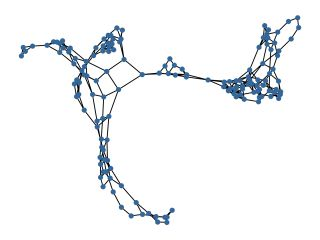
\includegraphics[scale=4]{protein.jpg}
\caption{Graf proteina}
\label{fig:protein}
\end{figure}
Nije odgovarala činjenica da je prikaz molekula proteina zapravo neusmjereni graf pa je matrica susjedstva čvorova simetrična, što je upola manje računskog posla od onog koji bi bio potreban za naš projekt jer se uzima samo donji trokut u izračunima. Cilj našeg projekta je dobiti usmjereni graf. U radu se spominje kako je moguće napraviti preinake matrice, izračunati i gornji trokut. Također, zbog specifične forme dataseta, prilagodba na vlastiti dataset bila bi mukotrpna. Od pristupa se odustalo jer su pronađeni oni koji više obećavaju i kojima je potrebno manje prilagodbe. 

\section{Latent Skill Embedding (Lentil)}
\subsection{Općenito o Lentil-u}
%izvještaj prvog tjedna
Početno je istražen i opisan u {\color{red}Izvještaju prvog tjedna, staviti poveznicu na gornji dio teksta} \citep{6}. Daljnjim istraživanjem pokazuje velik potencijal. Metoda je upravljana podacima, uči reprezentaciju sadržaja koja ne zahtijeva \textit{a priori} znanje preslikavanja \textit{content-to-concept}. Proširuje ideje \textit{sparse factor analysis} (SPARFA) i multidimenzionalne Item Response Theory.\newline
Model uči prikaz korisničkog znanja, kao i edukacijski sadržaj kako bi se prikazale preporuke, personalizirane upute o učenju. Probabilistički je model. Problem je formuliran kao regularizirani \textit{maximum-likelihood embedding} korisnika, nastavnih cjelina (lekcija) i procjena znanja (ispita) u zajednički semantički prostor iz skupa podataka o prošlosti interakcije korisnik-sadržaj (\textit{access traces}). Nastavne cjeline i procjene znanja su moduli sadržaja. Fiksni su, a korisnici imaju putanje latentnim prostorom vještina. Stvara se multidimenzionalno okružje - studentsko znanje “leži” u kontinuiranom prostoru stanja, a preduvjeti lekcija moduliraju dobitke znanja lekcijskih modula. Ugradnja u taj prostor ne koristi simetrične udaljenosti komponenata, već se bilježi prirodni napredak težine procjene znanja i rasta korisničkog znanja.\newline
Korisnik je prikazan kao skup latentnih vještina, nastavna cjelina kao vektor dobitaka vještina i skupa preduvjeta, a procjena znanja kao skup potrebnih vještina. Korisniku se procjenjuje znanje nekog modula (ne zna ili zna, 0 ili 1), a vjerojatnost da će proći je veća ako korisnik ima visoku razinu vještine koja nadmašuje potrebne vještine za procjenu. Korisnik može poboljšati vještinu vremenom (koje je diskretizirano). Naglašava se da bi za poboljšanje vještine trebalo gledati korisničko predznanje (ovisno o predznanju podešavati težine u jednadžbi modela). 

\subsection{Ideje}
U radu je istražena i implementirana ideja određivanja slijeda lekcija pri praćenju znanja što se ispostavilo kao veoma primjenjivo na naš problem. Temelj eksperimenata s ovim modelom bila je vizualizacija slijeda zadataka. U kasnijoj etapi projekta, povratkom na ovaj obećavajući model, u originalni se kod implementiralo grupiranje zadataka kada su poznate pripadnosti koncepata i zadataka. Velika početna prednost modela je što koristi pronađeni Assistments dataset koji je prvi pronađen u skupu projekta i koji služi kao glavni temelj za usporedbu. Razmišljalo se na koji način je prigodnom veličinom dataseta moguće osigurati dovoljnu varijabilnost puteva učenja. \newline
U originalnim .ipynb bilježnicama primijećene su mnoge instance korisničkih putanja koje dijele iste lekcijske module na početku i module procjene na kraju, ali se sastoje od različitih lekcija tijekom učenja → stvaraju se mjehurići, \textit{bubbles}, koji su zapravo eksperimentalni dokaz dobrih svojstava različitih pristupa učenju. Mjehurići se koriste za evaluaciju sposobnosti ugradnje preporuke slijeda lekcija koja vodi do uspješnog ostvarenja ciljeva učenja. Model logističke regresije s L2 regularizacijom korišten za procjenu vjerojatnosti da će korisnik slijediti preporučenu “granu” mjehurića. Unutar svakog mjehurića, korisnici koji su krenuli preporučenim putem spojeni su s najbližim susjedom iz grupe onih koji nisu slijedili preporučeni put prema razlici u \textit{propensity scoreu}.

\subsection{Problemi i zadaci}
Kao početni potencijalni problem izvedbe modela pokazala se činjenica da su ocjene znanja modelirane na različitim osima grafičkih prikaza što za sobom povlači neovisnost lekcija i vještina, što ne mora u stvarnosti biti slučaj. Također, u prikazu putanja, u originalnim ispitnim podacima u radu vidljiva je pristranost korisničkih putanja jednoj vrsti temeljne, česte putanje zbog sličnosti pozadinskog znanja ispitanika.\newline
Isto tako, pronađena je greška u originalnom kodu; činjenica da se prijeđene putanje korisnika ne broje na odgovarajući način (iteriranje liste tupleova bezuspješno, uvijek 0).\newline
Pri početnom ostvarivanju vizualizacije slijeda zadataka kao problem je okarakterizirana činjenica da crta vektore, a ne pravi graf koji “povezuje” korisnike preko procjena ovisno o vještinama dobivenih nakon neke lekcije (više ukazuje na smjer potencijalnog puta, što isto donekle odgovara cilju projekta).\newline 
Izrađena je prilagodba na Google Colab, koja se pokazala izazovnijom od očekivanog zbog zastarjelosti originalnog koda i činjenice da je Google Colab službeno ukinuo podršku za Python 2.7 (iako je ipak i dalje moguće pokretati sadržaj).\newline
Nakon uspješne vizualizacije slijeda rješavanja zadataka Assistments dataseta, ideja je bila pokušati prilagoditi model našem "Biologija" datasetu. Potrebno je bilo riješiti problem prisutnosti varijabli trajanja i vremenskih koraka u originalnim funkcijama jer mi to ne gledamo i ne trebamo te spajati čvorove zadataka ovisno o pripadnosti pojedinom konceptu ili još bolje, spajati koncepte. 

\subsection{Rezultati}
Nakon početnog ispravljanja grešaka u kodu, dobiven je string koji označuje povezanosti čvorova dataseta na način da su strelicom povezani zadaci koje jedan korisnik rješava jedan za drugim prema pojavi u datasetu. Vizualizacija toga na cijelom datasetu generirala se preko 8 sati jer PyGraphviz, Pythonovo sučelje Graphviza (alata za crtanje grafova), ne iskorištava mogućnosti ubrazanja u Google Colabu. Odlučeno je prilagoditi i smanjiti dataset (uzeti prvih 200 redaka). Nakon toga uspješno je izvršena vizualizacija dvije vrste grafova koji prikazuju povezanost zadataka:
\begin{itemize}
\item graf tijeka (engl. \textit{flow grah}) - zadaci Assistment dataseta predstavljaju čvorove grafa koji se povezuju ovisno o korisničkom pristupu konkretnom problemu. Prikaz je vidljiv na slici ~\ref{fig:dot1}.
\item graf veza (engl. \textit{connection grah}) - čvorovi su i korisnici i zadaci kojima oni pristupaju. Prikaz je vidljiv na slikama ~\ref{fig:dot2} i ~\ref{fig:sfdp2}.
\begin{figure}[!htb]
\centering
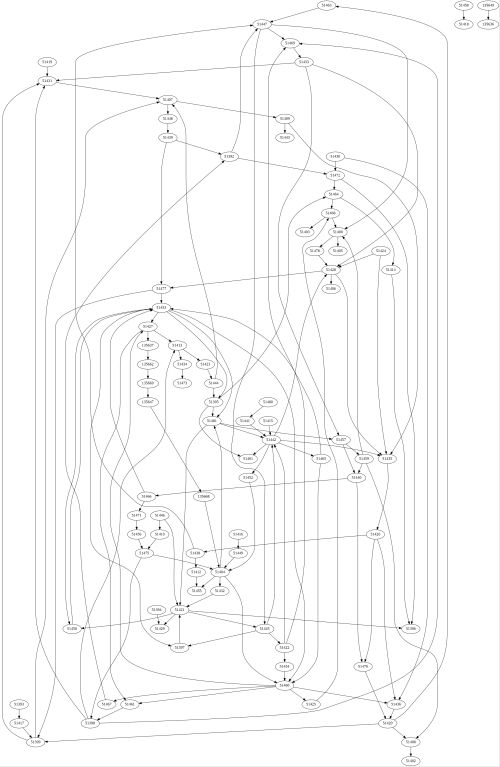
\includegraphics[scale=0.5]{dot1.jpg}
\caption{Originalni "dot" graf tijeka s podacima smanjenog Assistment dataseta}
\label{fig:dot1}
\end{figure}
\end{itemize}

\noindent Eksperimentiranjem s PyGraphvizom moguće je dobiti različite vizualne prikaze istog grafa (odnosno rasporede - dot, neato, twopi, circo, fdp, sfdp), pa je ovisno o namjeni moguće izabrati najprikladniji. Neki od prikaza vidljivi su na slikama ~\ref{fig:circo1} i ~\ref{fig:sfdp1}.

\begin{figure}[!htb]
\centering
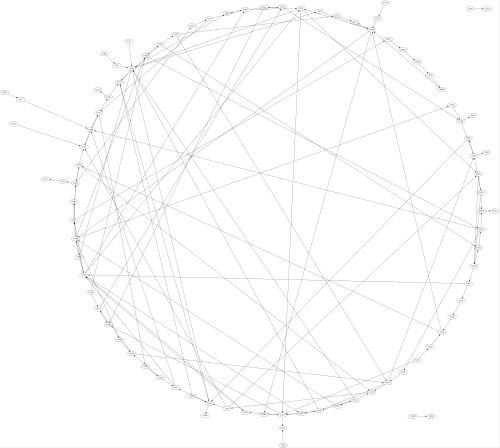
\includegraphics[scale=0.5]{circo1.jpg}
\caption{Originalni "circo" graf tijeka s podacima smanjenog Assistment dataseta}
\label{fig:circo1}
\end{figure}

\begin{figure}[!htb]
\centering
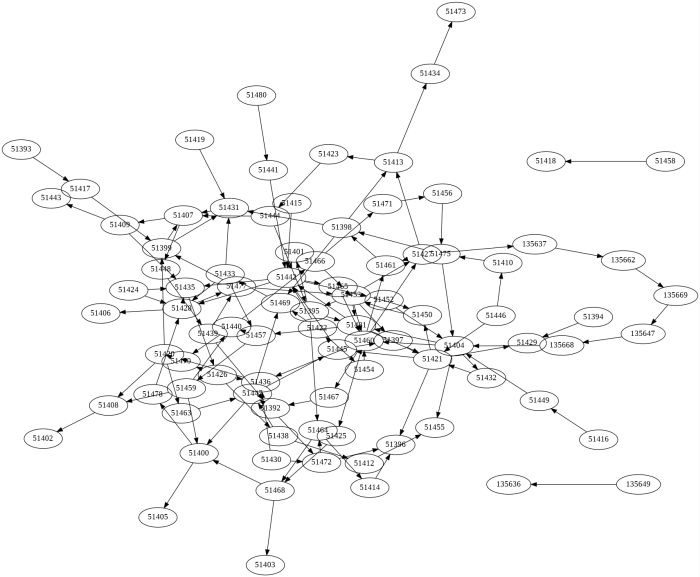
\includegraphics[scale=1.5]{sfdp1.jpg}
\caption{Originalni "sfdp" graf tijeka s podacima smanjenog Assistment dataseta}
\label{fig:sfdp1}
\end{figure}

\begin{figure}[!htb]
\centering
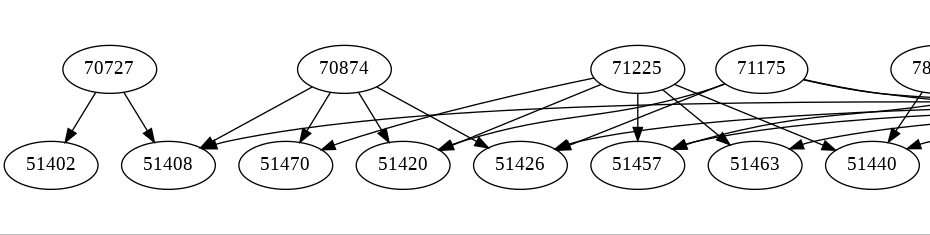
\includegraphics[scale=0.4]{dot2.png}
\caption{Originalni "dot" graf veza s podacima smanjenog Assistment dataseta}
\label{fig:dot2}
\end{figure}

\begin{figure}[!htb]
\centering
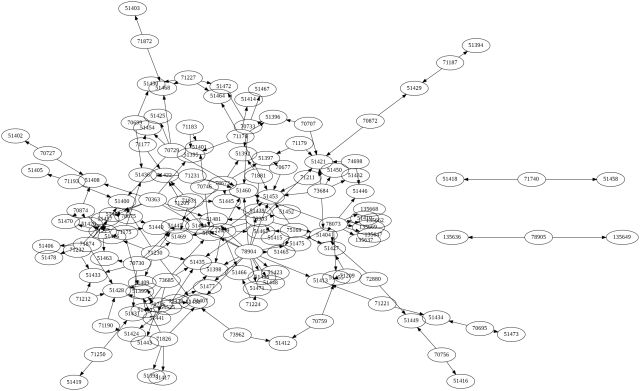
\includegraphics[scale=2]{sfdp2.jpg}
\caption{Originalni "sfdp" graf veza s podacima smanjenog Assistment dataseta}
\label{fig:sfdp2}
\end{figure}

\noindent Nakon ovakvog prikaza moguće je bilo zaključiti prednosti i nedostatke pojedine vrste prikaza.\newline
Graf veza mnogo je manje intuirivan i manje pregledan od grafa tijeka. Za daljnje eksperimentiranje, kao prikladniji graf uzet je graf tijeka zbog veće preglednosti i veće prilagođenosti našem problemu. No, iako je preglednost znatno bolja nego kod grafa veza, svejedno nije u potpunosti zadovoljen kriterij preglednosti. Zadaci različitih korisnika nisu obojeni različitim bojama, a ni pristup samim zadacima nije kronološki.\newline
Za intuitivniju vizualizaciju putanja dodane su oznake pojedinih korisnika između čvorova, što je vidljivo na slici ~\ref{fig:dot3}. Ideja je poboljšati dodavanjem različitih boja svakom korisniku. 

\begin{figure}[!htb]
\centering
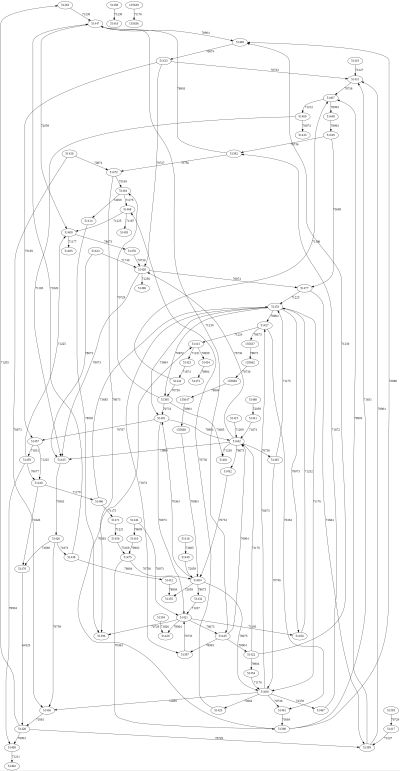
\includegraphics[scale=1]{dot3.jpg}
\caption{"dot" graf tijeka s podacima smanjenog Assistment dataseta uz dodane oznake korisnika}
\label{fig:dot3}
\end{figure}

\chapter{Clustering}
Početno se razmatralo na osnovu čega bismo u modelu preporuka mogli napraviti ostvarenje vizualizacije grupiranja (engl. \textit{clustering}) zadataka u koncepte ako nemamo označenu eksplicitnu pripadnost. Kao moguća ideje spominjao se redoslijed rješavanja, no zbog nerealnosti takve situacije najbrže je odbačena. Dodatno, moglo bi se gledati točnost pojedinih odgovora velikog broja ispitanika.
%-napravimo neku dodatnu varijablu mastery_score koja raste s točno riješenim zadatkom pa pratimo prema tome

\section{Latent Skill Embedding (Lentil)}

\noindent Nakon kratkotrajnog napuštanja Lentil modela zbog bavljenja modelima koji više obećavaju, napravljen je povratak u sklopu istraživanja za zadatak grupiranja zadataka ako nemamo eksplicitno definiranu pripadnost konceptima.\newline
Prvo je istražena mogućnost vizualnog grupiranja zadataka u okviru Lentil koda ako imamo pripadnost konceptima. Takva vizualizacija služila bi za usporedbu točnosti s modelom koji bismo osmislili. To je uspješno izvršeno. Dodan je stupac informacije o konceptima dataseta Assisstments u kod. Smanjenom datasetu za probu (20 pitanja) dodijeljene su različite oznake koncepata te je izvršeno grupiranje zadataka po konceptima izmjenom funkcije koja stvara graf tijeka manipulacijama s Pandasom (čvorovi su zadaci, na vezama oznake korisnika koje su ih riješile). Vizualizacija se nalazi na slici ~\ref{fig:clust1}.

\begin{figure}[!htb]
\centering
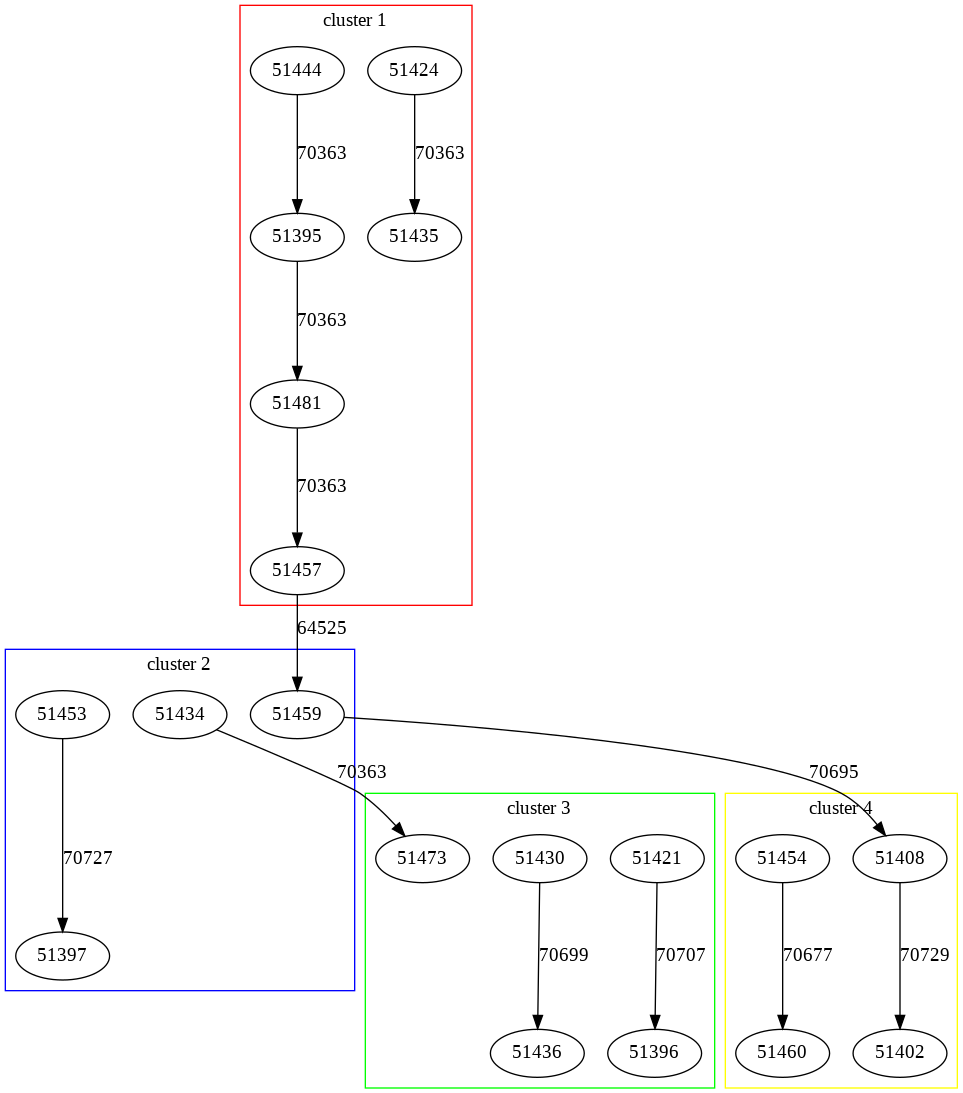
\includegraphics[scale=0.3]{clust1.png}
\caption{Grupiranje zadataka smanjenog Assistments dataseta prema pripadnosti konceptima}
\label{fig:clust1}
\end{figure}

\noindent Isti rezultat dobiven eksperimentom s drugačijim pristupom (izračunom matrice prijelaza između stanja (čvorova) Markovljevog modela). Grupiranje zadataka je identično kao na slici ~\ref{fig:clust1}, ali je prikaz manje interpretabilan jer u ovoj fazi ne prikazuje oznake korisnika. Vidljiv je na slici ~\ref{fig:clust2}.\newline
Konkretno, koristi se provjera različitosti pojedinih pitanja. Svaki zadatak teorijski je modeliran kao stanje Markovljevog procesa (diskretni stohastički proces je Markovljev proces ako vjerojatnost prijelaza u određenom diskretnom trenutku ovisi o stanjima u svim trenutcima prije). Stvara se matrica prijelaza između stanja (čvorova koji predstavljaju pitanja). Na osnovi takve matrice crta se graf. Kasnije se računa matrica vjerojatnosti prijelaza stanja pa stacionarna distribucija (vjerojatnosna distribucija koja se ne mijenja u Markovljevom lancu kako vrijeme prolazi). \newline
Ponovno čitanje rada \citep{6} inspiriralo je za ideju korištenja izračuna entropije za određivanje koncepata. Entropija se računa kao negativni skalarni produkt stacionarne distribucije i $Plog(P)$, gdje $P$ predstavlja matricu vjerojatnosti prijelaza među stanjima. Sama korist izračuna entropije još nije prikazana. Entropija inače predstavlja “porast informacije u podatcima”. Potencijalno, ideja je da, s obzirom da se računa za svaku matricu vjerojatnosti prijelaza, za svaku putanju različitih korisnika računati entropiju i utvrditi postoje li pravilnosti koje pomažu odrediti koncepte. 

\begin{figure}[!htb]
\centering
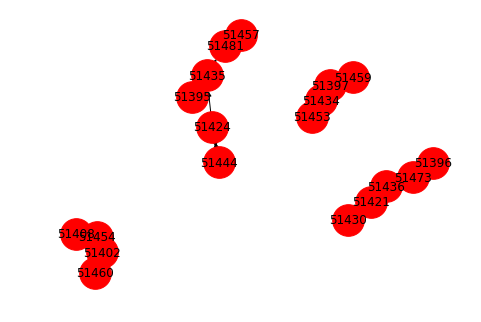
\includegraphics[scale=0.5]{clust2.png}
\caption{Grupiranje zadataka smanjenog Assistments dataseta prema pripadnosti konceptima izračunom matrice prijelaza}
\label{fig:clust2}
\end{figure}

\section{K-Medoids}
Kao odvojeni pristup, napravljena je skripta koja radi clustering pomoću algoritma K-Medoids.\newline
Kao vektor, odnosno element dataseta koji treba grupirati, uzeta je lista odgovora svih ispitanika na određeno pitanje (jedan element predstavlja jedno pitanje). Za metriku udaljenosti napravljena je funkcija koja gleda sumu razlika dva vektora (gleda se razlika između $x[i]$ i $y[i]$ za $i \in [0, broj ispitanika-1]$). Može se uzeti i kvadratni korijen te sume.\newline
Definirana je i funkcija koja računa grešku kao sumu elemenata koji nisu dobro grupirani. Uzeto je da je “prava” klasa ona kojoj pripada najviše elemenata iz tog koncepta, a oni koji nisu u njoj pridodani su ukupnoj sumi greške. 
Grupiranje se radi na standardiziranim i nestandardiziranim podacima i za obje verzije računaju se \textit{rand index}, \textit{adjusted rand index}, NMI vrijednost (\textit{normalized mutual information}) te ranije spomenuta funkcija koja računa broj krivo grupiranih primjera.\newline
Napravljena je i funkcija koja metodom lakta određuje idealan broj klasa, u slučaju da on nije otprije poznat.
\newline
\newline
Za različite datasetove skripta pokazuje funkcionalnost na različite načine.\newline
Biologija dataset:\newline
Za sad je algoritam isproban samo na datasetu Biologija (84 odgovora) jer je Assistments malo prevelik, ali sljedeći korak je testiranje i na Assistments.\newline
Dataset ima 30 pitanja, znači imamo 30 ulaznih vektora. Algoritam je isproban na standandiziranim i nestandardiziranim podacima, te daje nešto malo bolje rezultate na nestandandiziranim, ali to može biti i do dataseta. 
Rand index na nestandardiziranim podacima je 0.83, a adjusted rand index 0.41, za što kažu da spada u “srednje dobar rezultat”. NMI vrijednost je oko 0.58, a minimum koji se dobiva funkcijom za sumu greške jest 9 (od ukupno 30 pitanja). Lošiji rezultati mogu biti i do dataseta Biologija koji je svakako daleko od idealnog, jer ni koncepti nisu dobro definirani (npr. ispitanik možda ne zna živčanu stanicu, ali je čuo odgovor na par pitanja iz psihologije). 
Korištenjem metode lakta za određivanje broja klasa dobije se 6 klasa, dok je pravi broj klasa 5.\newline
Assistments dataset:\newline
Testiranje na Assistments u početku je okarakterizirano kao nemoguće jer K-Medoids algoritam zahtijeva da su svi vektori iste dimenzionalnosti odnosno da su svi ispitanici odgovorili na sva pitanja. To u Assistments nije zadovoljeno. Eventualno se može probati s nekakvom redukcijom dimentionalnosti vektora (npr. \textit{principal component analysis}, međutim budući da ima pitanja na koja je samo jedan student odgovorio, na kraju bismo trebali završiti s dimenzionalnošću 1 (što je puno premalo da bi obuhvaćalo potrebne informacije).\newline
U nastavku rada na ovom pristupu, napravljena je prilagodba za učitavanje smanjenog Assistments dataseta (20 pitanja). No, početna pretpostavka da testiranje s Assistemntsom neće biti moguće pokazala se ispravnom. Isprobana je metoda grupiranja slična K-Medoids, K-Means, ali nije pokazala željenu funkcionalnost.

\section{Ostatak istraživanja}
Mnogi radovi pokazali su se u cjelovitosti ne toliko relevantnima da bismo ih mogli u potpunosti primijeniti na naš problem, ali su predstavili mnoge iskoristive koncepte i algoritme vrijedne spomena.\newline
\newline
U radu \citep{ct10} spominje se da je razumijevanje krajnjeg cilja svakog studenta praćeno pomoću posebne varijable mastery\_score koja se osvježava svaki puta kada se vrši procjena studentovog znanja. \newline
Spominje se da identificiraju i vizualiziraju grupe povezanih koncepata. Točnije, \textit{spreading algorithm} pronalazi uzorak u povezanosti koncepata i dokumenata te dokumenata i koncepata. Analizirana je struktura \textit{spreading algorithma} \citep{ct11}.\newline
Problem je što je potrebna neka vrsta reference, ekspertno određenog početnog grafa koji će se evaluirati tim algoritmom.\newline
\newline
U radu \citep{12} predstavljene su hijerarhijske veze pitanja i koncepata modelirane pomoću hinge loss skalarnog produkta ugrađenih koncepata i pitanja. Problem: povezanost koncepata i pitanja određena ekspertima i zapisana u matrici ugradnje, a eksperte želimo izbjeći. Korišten je t-distributed stochastic neighbor embedding (tSNE) algoritam.
tSNE je algoritam strojnog učenja za vizualizaciju; nelinearna tehnika za redukciju dimenzionalnosti. Koristi se za ugradnju visokodimenzionalnih podataka za vizualizaciju u niskodimenzionalni prostor (2 ili 3 dimenzije). Slični objekti su s visokom vjerojatnosti modelirani točkama koje su blizu u prostoru, a različiti objekti udaljenim točkama \citep{13}.
Problem: velika osjetljivost algoritma na promjenu parametara.\newline
\newline
Rad \citep{14} primarno radi poveznicu između samih koncepata, ali i između koncepata i objekata učenja (zadataka, primjera, itd.) uz pretpostavke da je broj objekata učenja poznat. Glavni problem i razlog napuštanja ovakvog modela je što se \textit{preprocessing} objekata učenja radi se pomoću \textit{text-mininga}. Isto tako, rad pretpostavlja da je netko nekad označio povezanost koncepata i objekata učenja pa da može koristiti tu referencu. Nad tom referencom oblikuje se tzv. \textit{contextual network} koja sadrži više vrsta čvorova. Za izračunavanje sličnosti koncepata koriste se dva načina: već spomenuti \textit{spreading activation algorithm} i \textit{PageRank with Priors}.\textit{ PageRank with Priors} koristi se kao kvantitativna mjera sličnosti čvorova prema nekom drugom čvoru. Čestu primjenu ima u sustavima kategorizacije.
U konkretnom primjeru, propagiraju se stvarne karakteristike modela domene znanja u eksplicitne veze među konceptima.\newline
\newline
U radu \citep{15} veoma je izraženo shvaćenje da mnogi radovi poistovjećuju koncepte i zadatke i to pojednostavljenje uzrokuje probleme.\newline
Prepoznaju da grafovi znanja ciljaju da predstave znanje u obliku grafova tripleta; triju činjenica - (početni entitet, veza, završni entitet).\newline
Razlikuju povezanost koncepta i zadataka, koncepata međusobno te zadataka međusobno. Ovisno o vrsti povezanosti, koriste različite funkcije gubitka.\newline
Koncepte enkodiraju kao sfere, a zadatke kao vektore u istom semantičkom prostoru.\newline
Metoda je evaluirana pomoću predikcije veza i klasifikacije tripleta. Potonja ocjenjuje točnost tripleta.
Predikcija veza predviđa početni ili završni entitet iz triplea, ovisno koji nedostaje. Algoritmu je potrebno dati rangirane preporuke zadataka, ne samo najbolji rezultat.
Sve mogućnosti se rangiraju kao moguće upopunjavanje traženog praznog mjesta prema udaljenosti u određenoj funkciji gubitka. Za evaluaciju koriste se dvije mjere:
\begin{enumerate}
\item srednja recipročna mjera svih točnih instanci (MRR) i
\item razmjer točnih zadataka koji rangiraju ne više od N (Hits@N).
\end{enumerate}
Glavni problem, kao i u većini istraženih metoda: znaju koliko je koncepata.\newline
\newline
Rad \citep{16} slične vježbe grupira u koncepte naziva “problem schemas”. Koristi se hierarchical graph neural network. Konkretno, ovdje je mreža dvoslojna: donji je sloj zadataka (svaki čvor je jedan zadatak), gornji je sloj problemskih shema. Povezanost zadataka i problemskih shema modelira se \textit{assignment matrixom} koji se dobije pomoću \textit{hierarchical clustering analysis (HCA)}. HCA je metoda analize grupiranja bez nadzora korištenjem aglomerativnih ili divizivnih strategija za izgradnju hijerarhije grupa.
Za konstrukciju hijerarhijskog grafa zadataka spominje se iskorištavanje semantičke informacije zadataka i shema, ali kasnije se  spominje treniranje mreže samo pomoću HCA pa je i to jedan od pristupa koji valja detaljnije istražiti.\newline
\newline
Istražen je i alat Ampligraph \citep{17, 18}. Površna analiza definirala ga je kao dosta moćan alat. Funkcionalnosti obuhvaćaju stvaranje grafa znanja, treniranje ugradbenog modela na tripletima, evaluaciju modela, vizualno grupiranje pojmova.
Problem: s obzirom da koristi triplete (subjekt, predikat, objekt), potrebno je poznavati povezanost pitanja.


\chapter{Literatura}
\renewcommand{\bibsection}{}
\begin{thebibliography}{99}
\bibitem[1]{ct1} \url{https://www.analyticsvidhya.com/blog/2019/10/how-to-build-knowledge-graph-text-using-spacy/}
\bibitem[2]{ct2} K12EduKG, \url{https://aic-fe.bnu.edu.cn/docs/20181205101832069569.pdf}
\bibitem[3]{ct3} Deep Generative Models, \url{https://arxiv.org/abs/1803.03324}
\bibitem[4]{ct4} \url{https://eigenfoo.xyz/deep-autoregressive-models/}
\bibitem[5]{ct5} Graph Recurrent Attention Networks, \url{https://arxiv.org/abs/1910.00760}
\bibitem[6]{ct6} Latent Skill Embedding (Lentil), \url{https://arxiv.org/pdf/1602.07029.pdf}
\bibitem[7]{ct7} \url{http://math.ubbcluj.ro/~tradu/TI/coverch4_article.pdf}
\bibitem[8]{ct8} \url{https://www.slideshare.net/bamparopoulos/entropy-based-measures-for-graphs}
\bibitem[9]{ct9} \url{https://www.educationaldatamining.org/EDM2015/proceedings/short360-363.pdf}
\bibitem[10]{ct10} \url{https://www.researchgate.net/publication/333828640_INTERACTIVE_LEARNING_IN_A_CONVERSATIONAL_INTELLIGENT_TUTORING_SYSTEM_USING_STUDENT_FEEDBACK_CONCEPT_GROUPING_AND_TEXT_LINKING}
\bibitem[11]{ct11} \url{https://en.wikipedia.org/wiki/Spreading_activation}
\bibitem[12]{ct12} Deep Hierarchical Knowledge Tracing, \url{http://www.personal.psu.edu/ffm5105/files/2019/edm19.pdf}
\bibitem[13]{ct13} \url{https://en.wikipedia.org/wiki/T-distributed_stochastic_neighbor_embedding}
\bibitem[14]{ct14} Automatic Concept Relationships Discovery for an Adaptive E-course, \url{https://www.educationaldatamining.org/EDM2009/uploads/proceedings/simko.pdf}
\bibitem[15]{ct15} Differentiating Concepts and Instances for Knowledge Graph Embedding, \url{https://www.aclweb.org/anthology/D18-1222/}
\bibitem[16]{ct16} HGKT : Introducing Problem Schema with Hierarchical Exercise Graph for Knowledge Tracing, \url{https://arxiv.org/pdf/2006.16915v2.pdf}
\bibitem[17]{ct17} Ampligraph, \url{https://docs.ampligraph.org/en/1.3.1/}
\bibitem[18]{ct18} \url{https://github.com/Accenture/AmpliGraph/blob/master/docs/tutorials/ClusteringAndClassificationWithEmbeddings.ipynb}

\end{thebibliography}




\end{document}